\hypertarget{c5}{\chapter{État de l'art}}

Notre projet est constitué de plusieurs briques élémentaires dont il convient de comprendre
le fonctionnement et les alternatives qui existent. L'objectif de notre projet est de construire
un logiciel générant des bases d'apprentissage pour des reconnaisseurs d'écriture manuscrite.
Nous présenterons donc les différentes techniques permettant de réaliser cette tâche et en quoi
consistent les techniques sur lesquelles sont basés les reconnaisseurs d'écriture. Le langage de
programmation à utiliser dans le projet était libre : nous avons donc choisi le langage
\href{http://scala-lang.org}{Scala}, car il est un bon compromis entre la JVM, qui est notre zone
de confort et qui permet d'utiliser toutes les bibliothèques Java dans le projet, et un paradigme
fonctionnel, agréable à utiliser et qui permet d'introduire une touche supplémentaire d'originalité
dans le projet. Les différentes technologies que nous avons étudiées font donc partie de l'écosystème
de ce langage de programmation.

\section{Techniques de reconnaissance d'écriture}

Cette partie de l'État de l'art s'appuie sur les travaux de thèse de Luc MIOULET\cite{mioulet:2015} sur les différents
systèmes de reconnaissance d'écriture, et sur les travaux d'Adeline GRANET, Emmanuel MORIN, Harold MOUCHÈRE,
Solen QUINIOU et Christian VIARD-GAUDIN sur la reconnaissance de documents historiques\cite{rececr:2017}. Le cadre de notre
projet ne comprend pas le développement d'un reconnaisseur. Cette partie fera l'objet d'une collaboration
entre Doptim et l'équipe IntuiDoc dans le cadre d'une thèse. Il est cependant intéressant de comprendre
les mécanismes sur lesquels ceux-ci sont basés.

\paragraph{}
Afin de tester notre logiciel, nous utiliserons le système de reconnaissance Laia. Cet outil permet
de créer des modèles de reconnaisseurs d'écriture manuscrite en \textit{deep learning}. Il nous
faudra donc utiliser leur modèle de reconnaisseur, l'entraîner sur une base d'apprentissage que nous aurons
générée avec notre logiciel, et nous verrons si les résultats obtenus avec ce modèle sont bons ou non. 

\paragraph{}
La plupart des techniques de reconnaissance de l'écriture sont basées sur des classifieurs
dits dynamiques, c'est-à-dire qu'ils possèdent une mémoire interne ou possèdent une notion
de contexte dans leur analyse. Ces classifieurs permettent un parcours et une division des
données d'entrée et donc d'effectuer une classification pour chacune des divisions repérées. 
		
\subsection{Modèles de Markov Cachés}

Les Modèles de Markov Cachés (MMC) sont des modèles probabilistes basés sur une structure de
graphe d'états. Ils modélisent une séquence basée sur des connaissances \textit{a priori},
comme un langage pourrait être défini à l'aide de la forme des lettres. Les probabilités de passage
d'un état à un autre dépendent d'une matrice de transition et un vecteur de conditions initiales
permet de définir l'état de départ. Les MMC permettent de modéliser la probabilité de choisir un caractère
en fonction de l'état actuel du système de reconnaissance. Pour cela, les différentes composantes
de l'alphabet utilisé sont décomposées (première partie de boucle du \texttt{d}, barre verticale du \texttt{l}, \ldots).
Ces composantes correspondent aux états du graphe. On pourra donc modéliser la
probabilité pour un système de choisir un \texttt{l} après avoir lu une barre verticale, etc.
Ces probabilités ne seront pas égales à 1 car une barre verticale peut aussi correspondre à un
\texttt{t} par exemple. Cependant, cette approche impose une segmentation des composantes
de l'alphabet que l'on souhaite traiter et impose de changer ces composantes ou d'étendre
l'alphabet reconnu. Or, cette segmentation et l'étiquetage correspondant (\textit{e.g.} "c'est une boucle d'un a")
ne sont pas toujours évidents et peuvent être fastidieux à faire.

\paragraph{}
\begin{mdframed}[frametitle={Figure 8 : Schéma de transition et d'observation d'un MMC}, innerbottommargin=10]
\begin{center}
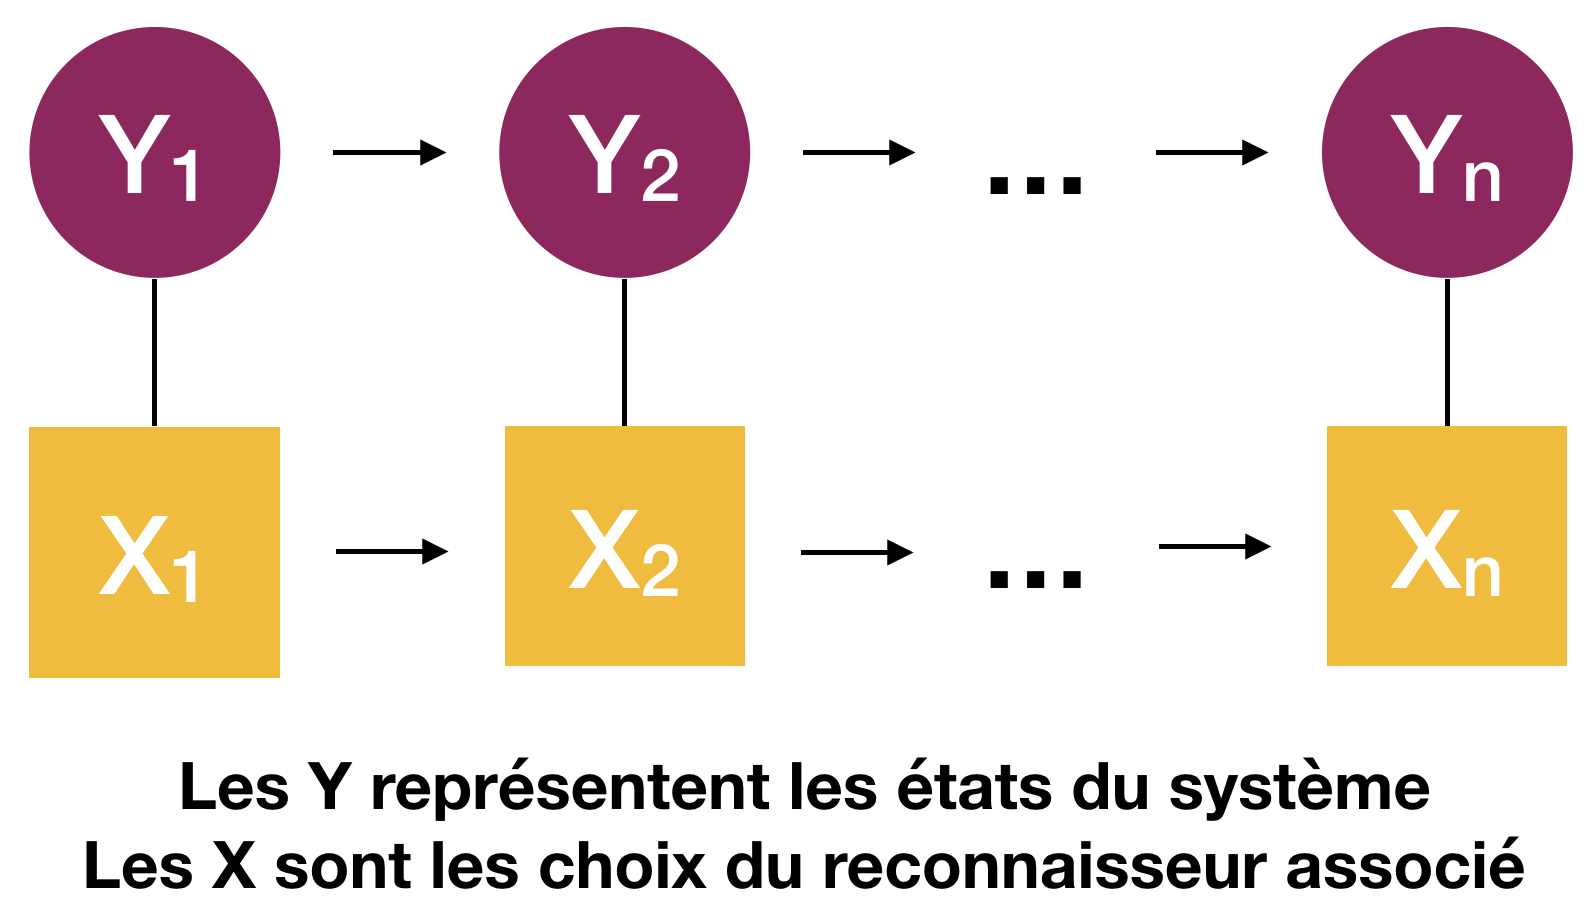
\includegraphics[width=0.6\linewidth]{mmc.png}
\end{center}
\end{mdframed}

\subsection{Champs Aléatoires Conditionnels}

Les Champs Aléatoires Conditionnels sont des modèles basés également sur des probabilités et
sur une structure similaire aux MMC. La principale différence entre ces deux méthodes est que pour les MMC,
les probabilités de choix des caractères dépendent d'un état, tandis que pour les CAC, le choix d'un
caractère peut être réalisé depuis n'importe quel état, avec une pondération par un potentiel.
Cette approche permet alors de prendre en compte l'ensemble du contexte local de la séquence observée
du fait de l'hypothèse de non-indépendance des états. Ce modèle est donc plus approprié pour l'analyse de
séquences structurées. Cependant, ils n'effectuent pas d'étiquetage de séquence lors de leur apprentissage,
et ne possèdent pas de structuration interne qui leur permettrait de saisir des structures de plus haut
niveau telles que les titres ou la date dans un document.

\paragraph{}
\begin{mdframed}[frametitle={Figure 9 : Schéma de transition et d'observation d'un CAC}, innerbottommargin=10]
\begin{center}
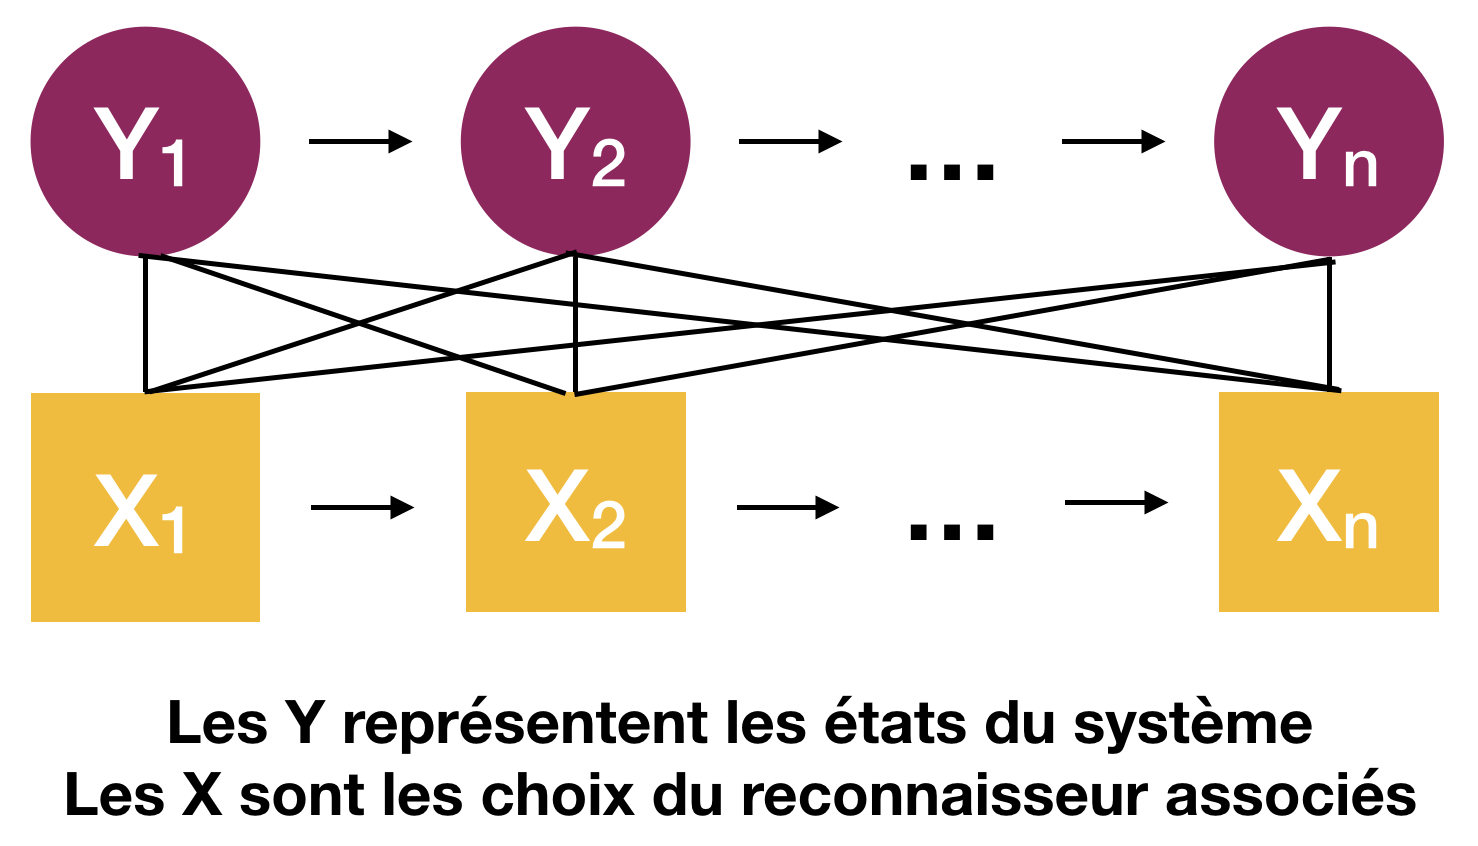
\includegraphics[width=0.6\linewidth]{cac.png}
\end{center}
\end{mdframed}

\subsection{Réseaux de Neurones Récurrents}

Les Réseaux de Neurones Récurrents sont basés sur la structure classique des réseaux de neurones,
avec une modification : chaque neurone des couches cachées possède également en entrée les sorties
des neurones correspondant à leur couche. Ceci permet d'avoir une mémoire interne des états de chaque couche.
Via cette approche, il n'est pas nécessaire d'effectuer un étiquetage des données car le réseau apprend
par lui-même. Cette méthode apporte également une vue plus globale de l'ensemble d'entrée car on ne se limite
pas à l'observation d'un état précédent. Le principal soucis de ces réseaux provient de l'apprentissage.
Ils nécessitent un grand jeu de données et on remarque une "disparition" du gradient sur les couches les plus
profondes, c'est-à-dire que les poids d'entrée ne sont que peu modifiés lors de l'apprentissage. Il faut alors
recourir à un apprentissage couche par couche, ce qui est compliqué à cause de la récurrence de ce type de réseaux.

\subsection{Réseaux de Neurones Récurrents Multi-Dimensionnels}

Les MDRNN sont conçus afin d'apporter une localité et une mémoire sur les deux dimensions de l'image traitée.
Ils sont constitués de couches de réseaux de neurones de différentes natures organisés selon l'abstraction des
données à effectuer. L'image est tout d'abord décomposée en blocs. Des réseaux récurrents la parcourent alors
en la transformant dans chaque direction diagonale. Les sorties de ces réseaux sont alors transmises à un
réseau convolutionnel qui permet d'augmenter le niveau d'abstraction des données de sortie. On fait ainsi
circuler les résultats des différents réseaux vers d'autres afin d'extraire de plus en plus d'informations
de haut niveau dans le document étudié.

\paragraph{}
\begin{mdframed}[frametitle={Figure 10 : Schéma de structure d'un MDRNN}, innerbottommargin=10]
\begin{center}
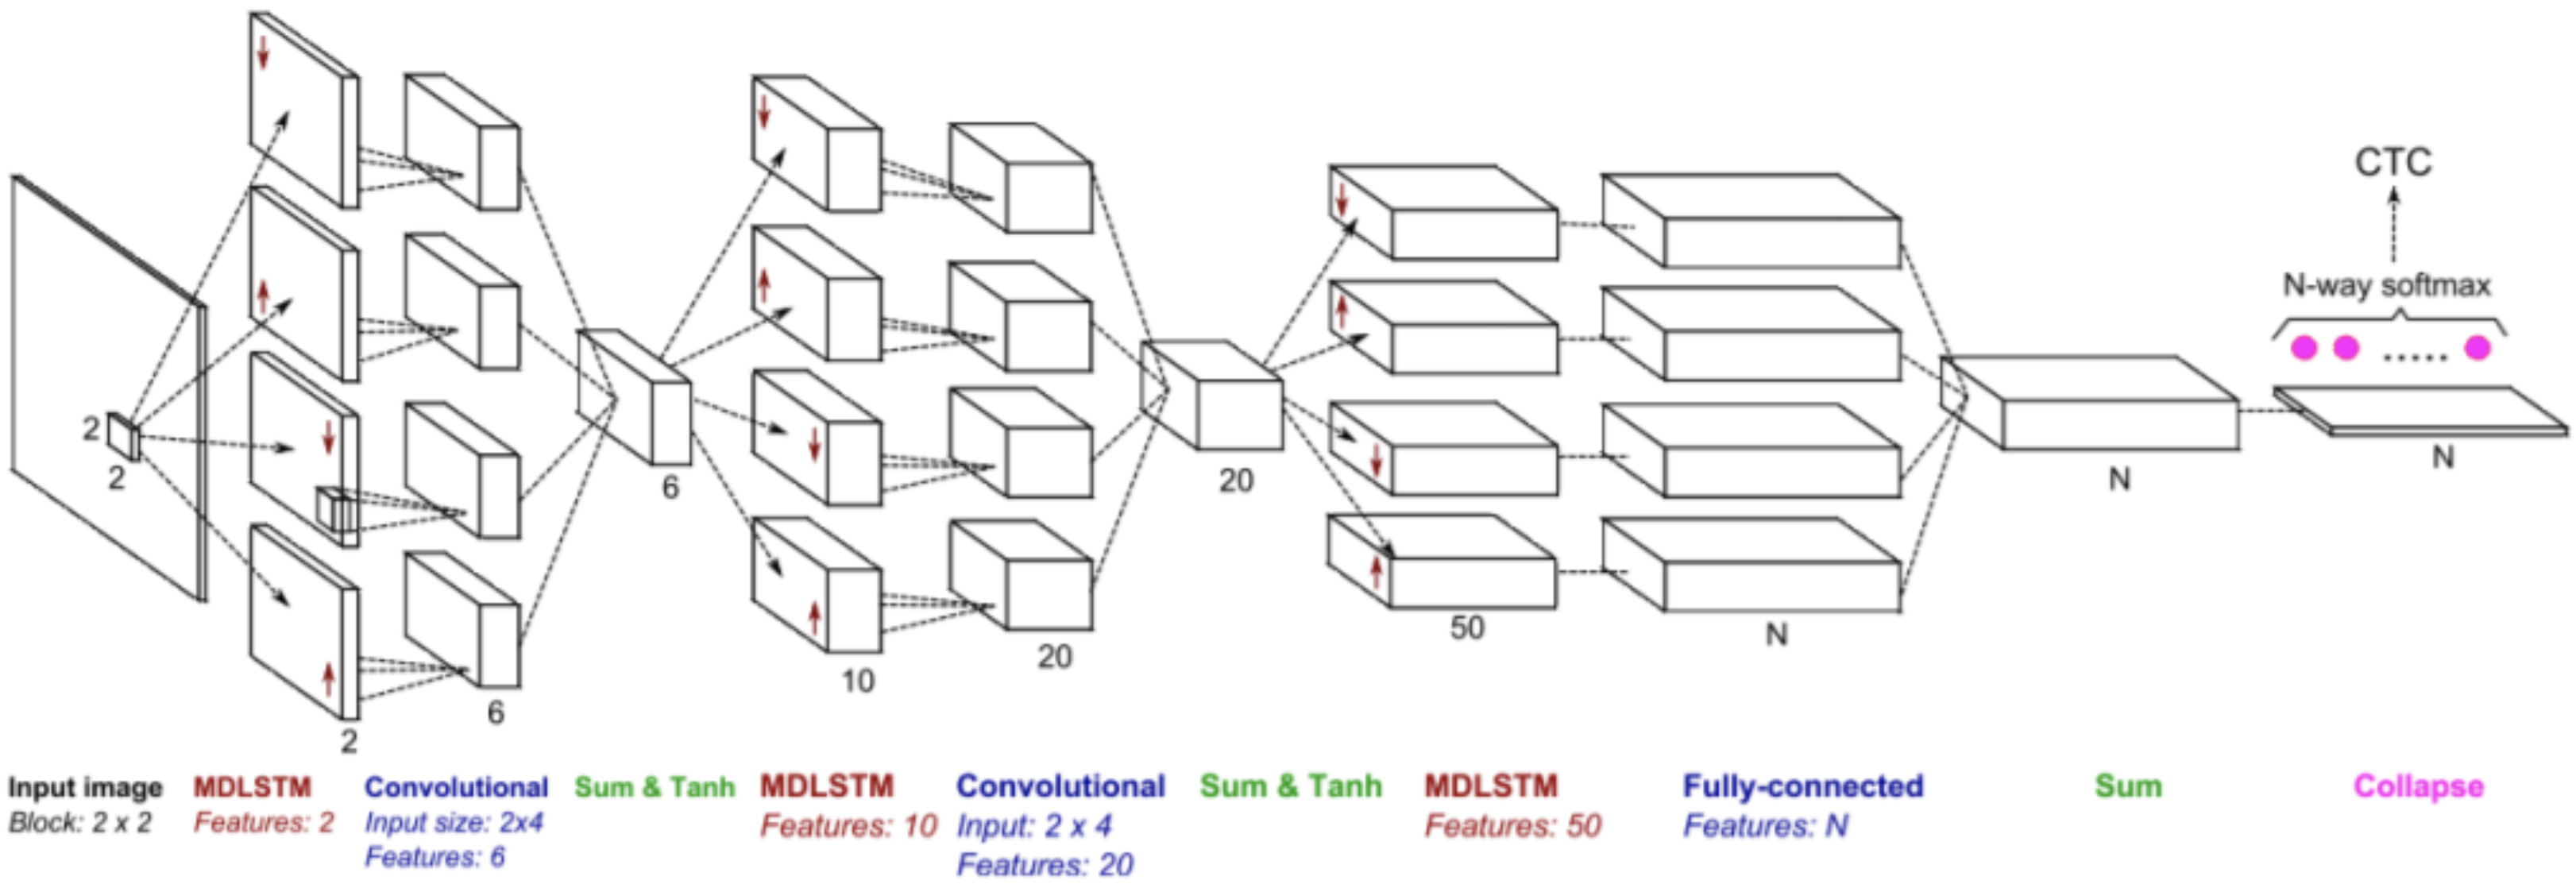
\includegraphics[width=0.6\linewidth]{mdrnn.png}
\end{center}
\end{mdframed}

\paragraph{}
Cependant, cette structure ne permet pas une segmentation de l'image de départ. Il est donc nécessaire de créer
cette segmentation afin d'établir une relation entre les données d'entrée et les sorties. Afin de réaliser cette
segmentation, une adaptation des algorithmes d'apprentissage est nécessaire.

\section{Détecteur de lignes}

Afin de pouvoir utiliser les techniques de reconnaissance manuscrite, il est d'abord nécessaire
de faire une segmentation des documents numérisés que nous possédons en entrée. La méthode
usuelle dans le domaine de la reconnaissance manuscrite est la segmentation par ligne des documents.
Pour ce faire, plusieurs techniques sont documentées dans la littérature concernant l'OCR
(\textit{Optical Character Recognition}). Cette partie s'appuie notamment sur une revue des différentes
techniques de segmentation parue dans l’\href{http://www.ijcsns.org/}{International Journal of Computer Science and Network Security}
par neuf membres de l’université de Malaya. La segmentation en lignes est une étape importante pour
la reconnaissance manuscrite puisqu'un mauvais découpage va inévitablement poser des problèmes
lors des étapes suivantes de la reconnaissance.

\paragraph{}
Il est alors important d'identifier les problèmes que pose la détection de lignes dans les documents manuscrits.
En effet, certains aspects sont à prendre en compte :
\begin{itemize}
\item les lignes fluctuent au sein d'un même document;
\item les lignes d'un texte ne sont pas espacées régulièrement;
\item certaines lignes peuvent se chevaucher;
\item l'espace interligne lui aussi peut varier d'une ligne à une autre et d'un paragraphe à un autre;
\item les lignes d'un paragraphe peuvent avoir une courbure globale et une courbure locale propre à
chaque ligne (et même locale à une partie d'une ligne).
\end{itemize}

\paragraph{}
Tous ces paramètres peuvent également différer entre deux paragraphes, deux textes, et deux écrivains. Nous allons maintenant
présenter rapidement les principales techniques documentées dans la littérature de l'OCR, pour ensuite décrire plus
précisément le fonctionnement des types de détecteurs de lignes que manipule l'équipe IntuiDoc. Nous tenons à préciser que
les détecteurs de lignes que nous utiliserons nous seront fournis et que nous n'aurons pas à en implémenter un.

\paragraph{}
Il existe globalement deux types d'approches pour la détection des lignes dans un document manuscrit : les approches
descendantes et les approches ascendantes. Les approches descendantes sont basées sur la technique de la projection.
La projection horizontale est appliquée au document ou à une partie du document. Ensuite, une analyse sur les \textit{maxima},
les \textit{minima} et les composantes connexes entre deux \textit{minima} consécutifs permettent de déterminer les lignes.
Les approches ascendantes sont basées sur le bas niveau (au niveau pixel ou composantes connexes). La classification
par K plus proches voisins (KNN), la transformée de Hough et la technique du lissage utilisent ce type d'approches.

\paragraph{}
Dans la classification par KNN, les alignements sont détectés en choisissant les composantes connexes, prolongées dans des
directions spécifiques, puis les lignes sont extraites en groupant ces alignements selon ces critères : proximité, similitude,
continuité de direction. Dans la transformée de Hough, les points sont les centres de gravité des composantes connexes.
Un ensemble de points alignés dans l'image et ayant un pic dans la transformée de Hough représente une ligne. Dans la technique
de lissage, les pixels noirs consécutifs sur la direction horizontale sont lissés. Les boîtes englobant les composantes connexes
dans l'image lissée forment les lignes. Nous allons maintenant voir plus en détail les techniques qui nous intéressent
dans le cadre de notre projet.

\subsection{Détection de lignes par réseau de neurones à convolution}

Pour la détection des lignes sur tout le document, un détecteur de lignes basé sur un réseau de neurones à convolution nous sera
fourni par IntuiDoc. Cette partie s'appuie sur un article\cite{crouspeyre:2017} de Charles CROUSPEYRE à propos du fonctionnement des
réseaux convolutifs, et sur les travaux de Sofia ARES OLIVEIRA, Benoît SEGUIN, et Frédéric KAPLAN\cite{} sur l’approche \textit{deep learning} de la segmentation
de documents. 

Les réseaux de neurones à convolution comparent les images fragment par fragment et recherchent des fragments caractéristiques.
Par exemple, un réseau de neurones à convolution cherchant à déterminer si une image est un X ou pas va chercher les caractéristiques
définissant les X, les diagonales et leur entre-croisement. Lorsqu'on lui présente une image, le système ne sait alors pas si les
caractéristiques sont présentes ni leur localisation. Il va alors calculer dans toute l'image si la caractéristique est présente.
Pour compléter une convolution, on répète ce processus alignant les caractéristiques à chaque sous-partie de l'image.
Le résultat de chaque convolution est une image stockant le résultat de la comparaison, avec un 1 pour une similitude et un -1
pour une différence par exemple. Ensuite, à partir du résultat de chaque convolution, on crée un tableau situant où les
caractéristiques se trouvent dans l'image. On obtient alors des images correspondant à l'image de base découpée en filtres.
On répète le processus de convolution pour chaque caractéristique, et on obtient alors la couche de convolution.

\paragraph{}
Cependant, le nombre d'opérations augmente linéairement avec le nombre de pixels de l'image et le
nombre de pixels de chaque caractéristique. On peut alors effectuer du \textit{pooling}. On va
réduire le nombre de pixels de l'image, en passant une fenêtre de quelques pixels sur l'image,
et dans laquelle on ne garde que la valeur qui nous importe. Ainsi, le réseau ne situe pas précisément
les caractéristiques dans l'image, il connaît seulement leur présence ou non. La couche de
\textit{pooling} sert simplement à diminuer la charge de calcul. En effet, on garde le même nombre
d'images avec les mêmes informations, mais le nombre de pixels est moindre.

\subsection{Détection de ligne par floutage}

Pour détecter les lignes sur un paragraphe, un détecteur de lignes par floutage sera utilisé. Cette partie s'appuie sur les
travaux d'Aurélie LEMAITRE, Jean CAMILLERAPP, et Bertrand COÜASNON sur la segmentation de textes manuscrits par l’utilisation
d’images floutées. Cette technique utilise la combinaison de deux niveaux d'analyse de l'image. Tout d'abord, une première
analyse bas niveau de l'image floutée est réalisée, ce qui est efficace pour les images à forte densité textuelle. Ensuite,
une analyse plus haut niveau est effectuée, ce qui est efficace sur des images à faible densité textuelle. La combinaison des
deux niveaux d'analyse permet de gérer les problèmes liés à la détection de lignes dans les documents manuscrits évoqués au
début de ce chapitre. L'analyse bas niveau de l'image floutée est composée de deux étapes que sont l'extraction de régions
noires dans l'image afin de construire des parties de l'axe de la ligne, ainsi que la construction de l'axe de la ligne.

\paragraph{}
\begin{mdframed}[frametitle={Figure 11 : Floutage d'une image}, innerbottommargin=10]
\begin{center}
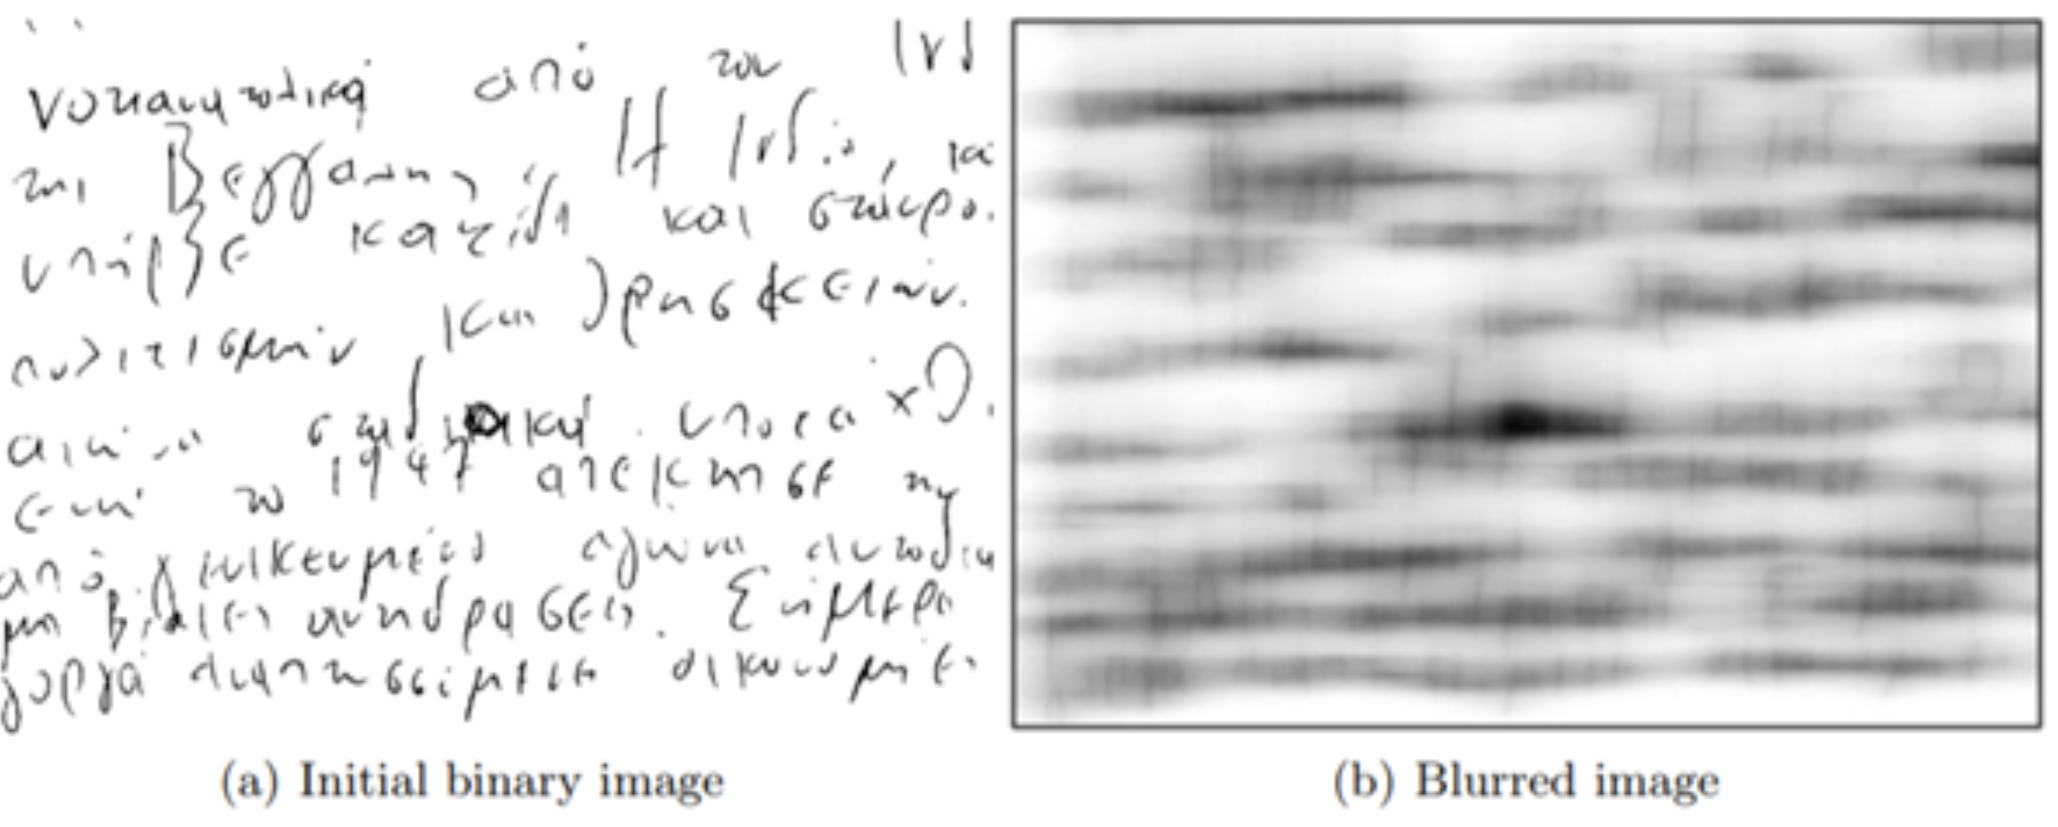
\includegraphics[width=0.6\linewidth]{detect1.png}
\end{center}
\end{mdframed}

\paragraph{}
Afin d'extraire les régions noires correspondant à des parties d'une ligne, il est nécessaire d'effectuer préalablement un
traitement sur l'image. Tout d'abord, l'image est floutée, puis une double binarisation lui est appliquée. Le résultat est
une image dans laquelle sont en évidence les « régions noires » qui vont être utilisées pour construire l'axe des lignes.

\paragraph{}
\begin{mdframed}[frametitle={Figure 12 : Binarisation d'une image}, innerbottommargin=10]
\begin{center}
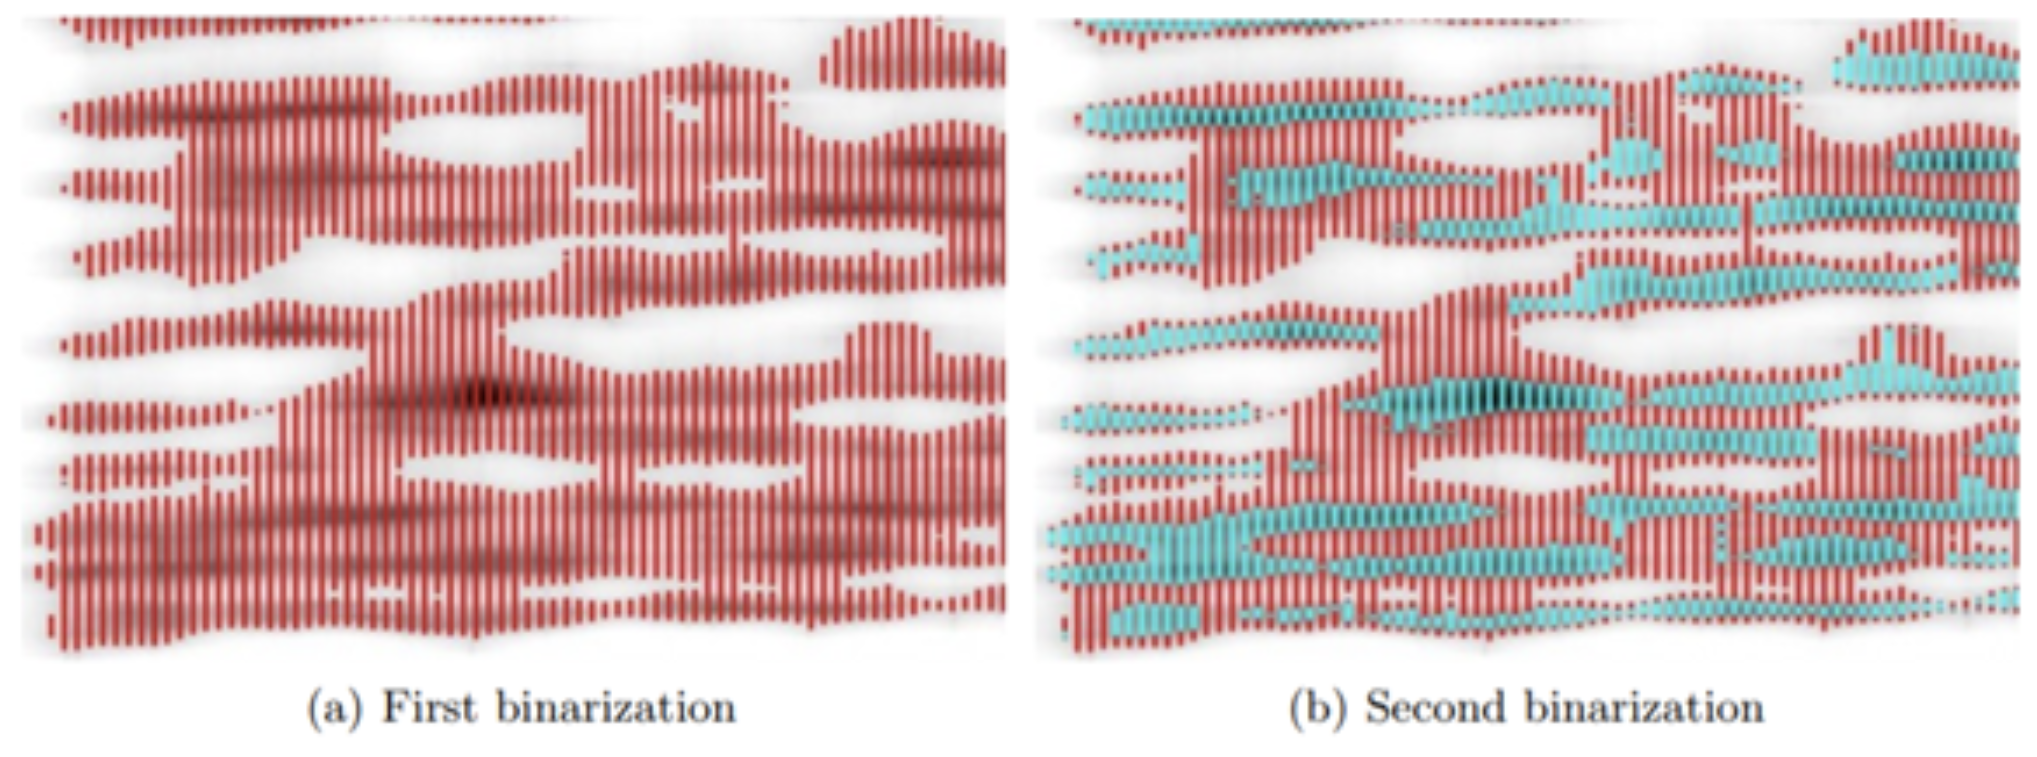
\includegraphics[width=0.6\linewidth]{detect2.png}
\end{center}
\end{mdframed}

\paragraph{}
Ces traitements d'image et la localisation de ces « zones noires » vont permettre ensuite de construire les axes des lignes.
Une analyse de la position et de l'épaisseur de ces zones va permettre de les relier entre elles. On pourra alors calculer
une épaisseur moyenne et une pente moyenne pour le document, données qui vont ensuite servir pour étendre les axes.

\paragraph{}
\begin{mdframed}[frametitle={Figure 13 : Extension des axes correspondant aux lignes de texte}, innerbottommargin=10]
\begin{center}
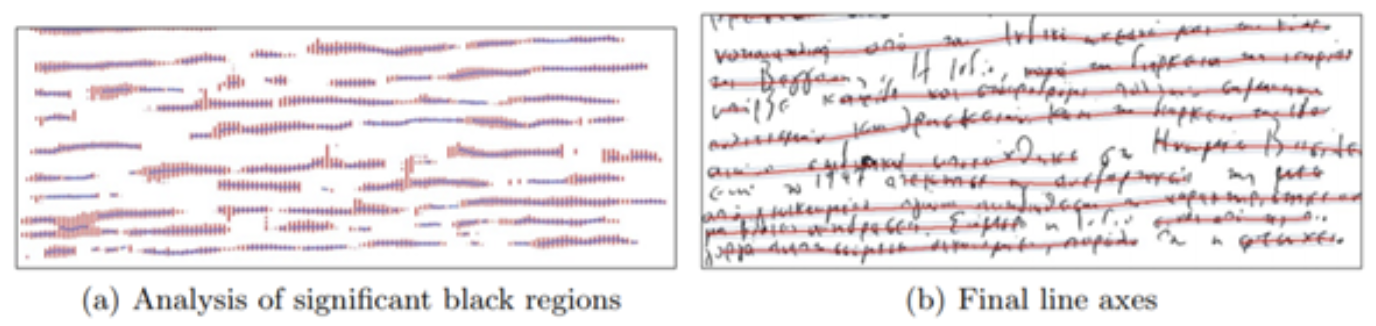
\includegraphics[width=0.6\linewidth]{detect3.png}
\end{center}
\end{mdframed}

\paragraph{}
En effet, la dernière opération de cette étape consiste à trier les différents axes créés. Des règles prenant en compte l'épaisseur,
la position et la pente des axes vont déterminer quels axes fusionner et quels axes supprimer. On peut obtenir des axes incomplets
en résultat de cette première analyse bas niveau. Cependant, aucune analyse supplémentaire ne peut être réalisée à ce niveau.

\paragraph{}
Le deuxième niveau d'analyse prend en compte le modèle du document étudié. À partir des différents axes de lignes créés dans l'étape
précédente, le but est de créer les lignes du texte. Ainsi, en fonction du document étudié, les stratégies de construction des lignes
seront différentes. Afin de spécifier un document, une description grammaticale basée sur deux types d'entités (les éléments connectés
et les axes créés précédemment) est effectuée. La description grammaticale du modèle du document va permettre de localiser les lignes
du texte et d'assigner des pixels à des lignes. Grâce à la description grammaticale et à des règles judicieusement choisies, on peut alors
construire les lignes du document. Cependant, il peut-être nécessaire (selon le domaine d'application) d'associer chaque pixel à sa ligne.
Une dernière analyse basée sur la description grammaticale du document couplée à certaines informations sur le document
est effectuée pour réaliser l'association.

\paragraph{}
Davantage d'informations sur ce sujet compliqué peuvent être obtenues en étudiant l'article\cite{cdbn:2009} donné en bibliographie.

\section{Format de description d'image}

\subsection{GEDI}

Le logiciel GEDI est un outil qui permet d'annoter des documents scannés. Il est ainsi très utile pour établir
la vérité terrain. Il met en scène deux types de documents : des images qui correspondent aux documents
scannés ainsi que des documents dans un format dérivé du XML auquel il donne son nom (le format GEDI), qui
permettent de stocker toutes les informations relatives aux documents scannés. On peut alors avoir, pour
chaque document scanné, des informations relatives à la position des paragraphes, à la langue dans laquelle
le texte est écrit, ou encore à la forme du texte (manuscrit ou imprimé). La vérité terrain que nous aurons
au sein de notre projet aura été établie avec GEDI.

\subsection{PiFF}

Le Pivot File Format (PiFF) est un format de description d'image basé sur JSON et créé par différents
chercheurs français : Harold MOUCHÈRE, Christopher KERMORVANT, Andres ROJAS, Mickal COUSTATY, Joseph CHAZALON
et Bertrand COÜASNON. C'est un format intermédiaire préalable au traitement d'une image dans le cadre
d'analyses de documents. Ce format est très utile pour l'analyse de documents puisqu'il permet le partage
de jeux de données, le traitement de résultats ainsi que l'utilisation d'outils déjà existants sans avoir à
faire de conversion entre les différents formats qui pourraient exister. De ce fait, les différentes étapes de
l'analyse de documents peuvent être effectuées par différentes équipes sans qu'il n'y ait de conflit au niveau
du format des données, ce qui permet une collaboration plus facile. Les données présentes en entrée dans le cas
de notre projet pourront se trouver sous différents formats, soit au format PiFF et dans ce cas il n'y aura rien
à changer, soit dans un autre format quelconque et il faudra alors les convertir. Les données de la base Maurdor
étant au format GEDI, il nous faudra notamment un convertisseur GEDI/PiFF. De ce fait, les données après traitement
par le logiciel seront toutes dans le format PiFF, ce qui permettra de les utiliser facilement.

\section{Base de données}

La question de la base de données est une question qui a été soulevée puisqu'elle constitue le pivot de notre
logiciel. En effet, elle centralise les couples imagette-retranscription produits lors du traitement des données
et est utilisée par tous les autres services. Tout d'abord se pose la question du stockage des images dans
une base de données. Il existe plusieurs façons de le faire. Il est possible de stocker l'image directement dans
une base de données SQL en binaire. Cependant, cette étape demande de transformer l'image pour l'insérer et de nouveau
pour la charger, ce qui peut poser des problèmes de latence s'il s'agit de grosses images ou s'il y a beaucoup
d'images à charger. Un autre moyen qui existe est de stocker non pas l'image mais une référence vers l'image,
soit son \textit{path}. Cette méthode, répandue en entreprise, a l'avantage de ne pas surcharger la base de données et
est souvent recommandée. Même si alors le poids de l'image ne pose plus problème, on n'accède plus à l'objet image en
lui-même, et cela impose de les stocker dans un serveur de fichiers hors de la base. Il existe également d'autres solutions
n'utilisant pas les bases SQL. En effet, les bases de type NoSQL permettent de stocker les images telles quelles du fait
de leur orientation document (on constitue des collections de documents que l'on lie). Ainsi, il serait possible d'intégrer
les images dans la base sans devoir les traduire dans un autre format.

\section{Interface Homme-Machine}

Les technologies existantes pour réaliser une IHM sont abondantes. Deux lignes de conduite s'offrent à nous. Nous pouvons
soit concevoir une application "lourde" comprenant une interface logicielle construite avec un outil du type de
\href{https://fr.wikipedia.org/wiki/JavaFX}{JavaFX}, soit créer une interface web. Nous devons gérer une base de données et
nous souhaitons que notre logiciel soit portable et puisse fonctionner sur un serveur. Nous avons donc préféré nous orienter
vers une implémentation web de l'interface. Cependant, il existe de multiples moyens d'utiliser une base de données avec une
application web. Nous pouvons par exemple utiliser des requêtes \href{https://en.wikipedia.org/wiki/Representational_state_transfer}{REST},
gérer la base de manière plus proche avec des scripts de type NodeJS ou PHP et construire l'interface en HTML/CSS et JS.
Il existe également des bibliothèques basées sur le modèle MVC, d'autres non. Nous avons isolé quatre frameworks web basés sur Scala :
\href{http://www.scala-js.org/}{Scala.js}, \href{https://www.playframework.com/}{Play},
\href{https://sourceforge.net/p/chaosuiframework/wiki/Home/}{Chaos} et \href{https://www.liftweb.net/}{Lift}. Scala.js est rapide,
fiable, facile à utiliser et utilise les bibliothèques JS existantes et une multitude d'autres bibliothèques standard.
Play est rapide, utilise \href{http://maven.apache.org/}{Maven} et la JVM, possède une communauté très active et propose un
rendu en temps réel. Chaos, très utilisé pour les applications REST, est léger, facile à prendre en main et utilise la JVM,
Scala et \href{https://jersey.github.io/}{Jersey}. Cependant, il n'est performant que pour les applications REST.
Enfin, Lift est principalement orienté vers les applications avec un fort besoin de sécurité. Il est rapide, facile à maintenir et
propose des modules pré-construits ainsi qu'une large documentation dont la qualité est néanmoins très variable. Ainsi, il nous
est nécessaire de définir les rôles et les objectifs de l'interface ainsi que les interactions qu'elle aura avec le reste du
programme afin de pouvoir déterminer l'approche et les technologies nécessaires.

\section{Traitement d'images}

Pour le traitement d'images, plusieurs bibliothèques logicielles sont à notre disposition. On peut citer
\href{https://github.com/python-pillow/Pillow}{Pillow}, \href{https://github.com/imagej/imagej1}{ImageJ},
\href{https://www.imagemagick.org/script/index.php}{ImageMagick} ou \href{https://opencv.org/}{OpenCV}.
Cette dernière nous a été conseillée par notre encadrant de projet, et elle est reconnue comme un
standard parmi les technologies de traitement d'images utilisées par la communauté, car elle elle est
disponible sur plusieurs plateformes et interfaçable avec plusieurs langages (C++, Java, Python, \ldots).
Elle convient donc parfaitement aux besoins que nous avons (compatibilité avec la JVM, bibliothèque complète et
\textit{cross-platform}). D'après le cahier des charges, nous n'aurons pas à utiliser ses fonctionnalités
les plus avancées (à base d'intelligence artificielle) au cours de ce projet, mais cela permet une fois de plus
que le projet soit évolutif, c'est-à-dire que les chercheurs qui maintiendront le projet pourront y ajouter
des éléments de traitement d'images plus avancés. Ce choix est donc validé dès maintenant.